%%%%%%%%%%%%%%%%%%%%%%%%%%%%%%%%%%%%%%%%%
% University/School Laboratory Report
% LaTeX Template
% Version 3.1 (25/3/14)
%
% This template has been downloaded from:
% http://www.LaTeXTemplates.com
%
% Original author:
% Linux and Unix Users Group at Virginia Tech Wiki
% (https://vtluug.org/wiki/Example_LaTeX_chem_lab_report)
%
% License:
% CC BY-NC-SA 3.0 (http://creativecommons.org/licenses/by-nc-sa/3.0/)
%
%%%%%%%%%%%%%%%%%%%%%%%%%%%%%%%%%%%%%%%%%

%----------------------------------------------------------------------------------------
%	PACKAGES AND DOCUMENT CONFIGURATIONS
%----------------------------------------------------------------------------------------

\documentclass[12pt]{article}

\usepackage[version=3]{mhchem} % Package for chemical equation typesetting
\usepackage{ctex}
\usepackage{siunitx} % Provides the \SI{}{} and \si{} command for typesetting SI units
\usepackage{graphicx} % Required for the inclusion of images
\usepackage{natbib} % Required to change bibliography style to APA
\usepackage{amsmath} % Required for some math elements

\setlength\parindent{0pt} % Removes all indentation from paragraphs

\renewcommand{\labelenumi}{\alph{enumi}.} % Make numbering in the enumerate environment by letter rather than number (e.g. section 6)

% \usepackage{times} % Uncomment to use the Times New Roman font

%----------------------------------------------------------------------------------------
%	DOCUMENT INFORMATION
%----------------------------------------------------------------------------------------

\title{MPI梯形积分实验报告} % Title
\author{劳马东 \textsc{16337113}\\数据科学与计算机学院\\计算机科学与技术(超算方向)} % Author name
\date{\today} % Date for the report
\begin{document}
\maketitle % Insert the title, author and date

\section{基本思想}
\qquad 梯形积分法可以用来估算函数f(x)、两条垂直于x轴的直线与x轴
围成的区域的面积大小。如下图1,其基本思想是:将x轴上的区间划分成n个等长的子区间,然后估算介于函数图像
及每个子区间内的梯形区域的面积。在n充分大时,子区间长度充分小,此时可以认为f(x)图像是一条
直线,于是可以用梯形的面积公式来计算。
\begin{figure}[h]
\begin{center}
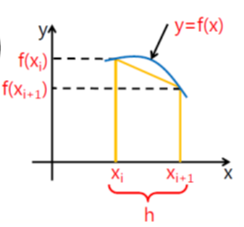
\includegraphics[width=0.35\textwidth]{p2.png} % Include the image placeholder.png
\caption{梯形积分法示意图}
\end{center}
\end{figure}
\newpage
\par \qquad 一个梯形的面积:
\begin{equation}
  A_i = \frac{h}{2}[f(x_i) + f(x_{i+1})],其中(h = \frac{b-a}{n}, x_i=a+i \times h)
\end{equation}
\par \qquad 总面积:
\begin{equation}
  \begin{aligned}
    A &= \sum\limits_{i=0}^{n-1}A_i \\
    &= \sum\limits_{i=0}^{n-1}\frac{h}{2}[f(x_i) + f(x_{i+1})]\\
    &=h[\sum\limits_{i=1}^{n-1}f(x_i) + \frac{f(a)+f(b)}{2}]
  \end{aligned}
\end{equation}

\begin{figure}[h]
\begin{center}
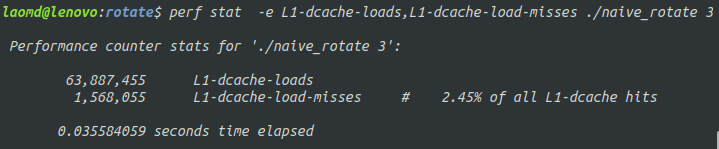
\includegraphics[width=0.8\textwidth]{p3.png} % Include the image placeholder.png
\caption{梯形积分法代码}
\end{center}
\end{figure}

\section{实验过程}
\subsection{任务划分}
假设将区间分为n个等长子区间和p个任务,则每个任务至少分得$\lfloor \frac{n}{p} \rfloor$
个子区间。考虑n不能整除p的情况,设余数为r。则这r个子区间分给前r个任务。因此,每个任务得到的
子区间数$f(i)$为:
\begin{equation}
f(i)=\left\{
\begin{array}{lll}
\lfloor \frac{n}{p} \rfloor + 1 & & {i = 0, 1, ..., r-1},\\
\lfloor \frac{n}{p} \rfloor & & {i = r, r+1, ..., p-1}.\\
\end{array} \right.
\end{equation}
每个任务起始的$a_i$为:
\begin{equation}
  \begin{aligned}
    a_i &= a+h\sum\limits_{j=0}^{i-1}f(j), i\in [0, p)\\
    &= \left\{
    \begin{array}{lll}
    a+h \times i(\lfloor \frac{n}{p} \rfloor + 1) & & {i = 0, 1, ..., r-1},\\
    a+h \times \{r(\lfloor \frac{n}{p} \rfloor + 1) + (i-r)\lfloor \frac{n}{p} \rfloor\} & & {i = r, ..., p-1}.\\
    \end{array} \right.
  \end{aligned}
\end{equation}
每个任务起始的$b_i$为:
\begin{equation}
  b_i = a_i + f(i) \times h
\end{equation}
\begin{figure}[h]
\begin{center}
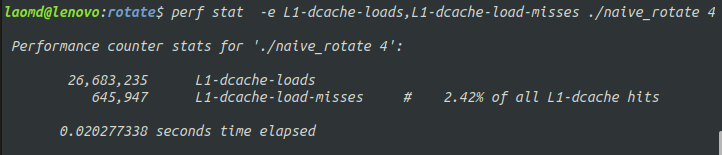
\includegraphics[width=\textwidth]{p4.png} % Include the image placeholder.png
\caption{任务划分代码}
\end{center}
\end{figure}
\subsection{任务间的通信}
采用master-slave通信模型,0号进程为master,其余进程为slave。
\subsection{任务聚合}
slave进程向master进程发送局部积分,master进程将受到的局部积分与自己的局部积分相加。
\section{测试结果}
测试函数$f(x)=\sin(x)$,n=2049,区间为$[0, \pi]$。如图4,估计结果为2=$\int_{0}^{\pi} \sin(x)$。
\begin{figure}[h]
\begin{center}
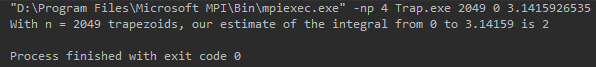
\includegraphics[width=\textwidth]{p5.png} % Include the image placeholder.png
\caption{任务划分代码}
\end{center}
\end{figure}
\end{document}
